\section{Speed Reading}
Speed reading is the act of trying to read faster than normal. There are various ways to read a given text, depending on the context and the purpose of the reading \cite{differentWaysOfReading}. \citeA{ziefle_effects_1998} has shown than when reading on paper, people read an average of 201 words per minute, and about 180 when reading on a monitor (depending on its resolution). Speed reading is all about raising one's words per minute. Numerous techniques have been utilized throughout the years, and  thanks to computers, reading software is becoming more available these days.


\subsection{Rapid Serial Visual Presentation (RSVP)}
Rapid Serial Visual Presentation is a technique that has become popular in the last few years. It's the idea of presenting words in small flashes, one at a time. In traditional reading, jumping from one word to another is done by saccading, which has a time penalty, since the eyes physically have to move back and forth. In RSVP, the goal is to eliminate saccading, thereby increasing reading speed. One of the more popular RSVP solutions is Spritz. According to their website, about 80\% of the time spent reading is used on physically moving the eyes from word to word \cite{spritz}.	It is claimed that by utilizing RSVP, it is possible to reduce this time. Additionally, by aligning the words according to the optimal recognition position, results can get even faster. Figure \ref{fig:spritz_orp} illustrates this concept. Spritz claims that it is possible to read up to 1000 words per minute \cite{spritz}.

\begin{figure}[htbp]
\centering
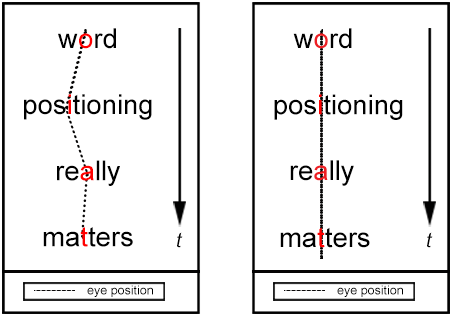
\includegraphics[width=0.4\textwidth]{Pics/opr_spritz}
\caption{Spritz utilizes the optimal recognition position to align words. \protect\cite{spritz}}
\label{fig:spritz_orp}
\end{figure}